\chapter{Fase A: Architectural Vision Phase}

\section{Pendahuluan}
Fase \textit{Architectural Vision} adalah langkah awal dalam Metode Pengembangan Arsitektural (ADM) TOGAF. Pada fase ini, tujuan utamanya adalah menetapkan lingkup dan arah proyek arsitektural secara menyeluruh. Fase ini melibatkan identifikasi pemangku kepentingan utama, pemetaan kebutuhan dan kekhawatiran mereka, serta definisi awal visi arsitektural yang akan memberikan panduan bagi pengembangan arsitektur secara keseluruhan.

Selain itu, fase ini bertujuan untuk mengembangkan pernyataan visi arsitektural yang mampu menyampaikan nilai bisnis dan kapabilitas yang akan dicapai oleh arsitektur enterprise yang diusulkan. Visi arsitektural ini menjadi dasar untuk menyusun \textit{Architectural Statement of Work}, yaitu dokumen kerja yang akan menjadi acuan dalam pengembangan dan implementasi arsitektur di fase-fase berikutnya. 

Persetujuan dari pemangku kepentingan terhadap \textit{Architectural Statement of Work} pada fase ini merupakan kunci keberhasilan, karena dokumen ini akan digunakan untuk memastikan bahwa semua pihak memiliki pemahaman yang sama terkait arah dan tujuan proyek arsitektural yang akan dilaksanakan.


\section{Tujuan}
\begin{itemize}
	\item Mengembangkan visi jangka panjang mengenai kapabilitas dan nilai bisnis yang akan dihasilkan dari arsitektur perusahaan yang diusulkan.
	\item Mendapatkan persetujuan untuk \textit{Architectural Statement of Work} yang mendefinisikan program kerja untuk mengembangkan dan mengimplementasikan arsitektur yang dijabarkan dalam \textit{Architectural Vision}.
\end{itemize}

\section{Input}
\begin{itemize}
	\item Permintaan Pekerjaan Arsitektur.
	\item Prinsip bisnis, tujuan bisnis, dan pendorong bisnis.
	\item Model Organisasi untuk Arsitektur Perusahaan.
	\item Kerangka Arsitektur yang Disesuaikan, termasuk prinsip-prinsip arsitektur.
	\item Repositori Arsitektur yang Terisi, seperti dokumentasi arsitektur yang ada (deskripsi kerangka kerja, deskripsi arsitektur, deskripsi baseline yang ada, dan sebagainya).
\end{itemize}

\section{Langkah-Langkah}
\begin{enumerate}
	\item Membuat proyek arsitektur.
	\item Mengidentifikasi pemangku kepentingan, kekhawatiran, dan kebutuhan bisnis.
	\item Memastikan dan mengembangkan tujuan bisnis, pendorong bisnis, dan batasan.
	\item Mengevaluasi kapabilitas bisnis.
	\item Menilai kesiapan untuk transformasi bisnis.
	\item Menentukan ruang lingkup.
	\item Memastikan dan mengembangkan prinsip-prinsip arsitektur, termasuk prinsip-prinsip bisnis.
	\item Mengembangkan \textit{Architectural Vision}.
	\item Menentukan nilai dari Target Arsitektur yang diusulkan dan indikator kinerjanya (KPI).
	\item Mengidentifikasi risiko transformasi bisnis dan kegiatan mitigasinya.
	\item Mengembangkan \textit{Architectural Statement of Work} dan mendapatkan persetujuan.
\end{enumerate}

\subsection*{Contoh langkah-langkah:}
\begin{enumerate}
	\item \textbf{Membuat proyek arsitektur.} 
	Proyek arsitektur untuk Hybrid Working di Universitas dimulai dengan menyusun tim proyek yang terdiri dari anggota fakultas, staf IT, dan manajemen. Tim ini bertugas untuk merancang arsitektur yang mendukung kerja hybrid, termasuk sistem manajemen ruang, perangkat lunak kolaborasi, dan kebijakan kerja.
	
	\item \textbf{Mengidentifikasi pemangku kepentingan, kekhawatiran, dan kebutuhan bisnis.} 
	Pemangku kepentingan utama termasuk dosen, mahasiswa, dan staf administrasi. Kekhawatiran utama meliputi aksesibilitas teknologi, kebutuhan ruang kerja fleksibel, dan keterlibatan mahasiswa dalam proses pembelajaran. Kebutuhan bisnis mencakup peningkatan efisiensi pengajaran dan pembelajaran serta dukungan untuk kolaborasi antar tim.
	
	\item \textbf{Memastikan dan mengembangkan tujuan bisnis, pendorong bisnis (\textit{business dri\-vers}), dan batasan (\textit{constraints}).} 
	Tujuan bisnis untuk implementasi Hybrid Working mencakup peningkatan partisipasi mahasiswa sebesar 20\% dalam kegiatan online. Pendorong bisnis termasuk kebutuhan untuk menarik lebih banyak mahasiswa dengan menawarkan fleksibilitas dalam cara mereka belajar. Batasan yang dihadapi meliputi anggaran terbatas dan perbedaan dalam kemampuan teknologi antar fakultas.
	
	\item \textbf{Mengevaluasi kapabilitas bisnis.} 
	Kapabilitas bisnis saat ini dievaluasi melalui survei kepada staf dan mahasiswa mengenai pengalaman mereka dengan pembelajaran jarak jauh dan fasilitas fisik. Hasil survei menunjukkan bahwa sebagian besar mahasiswa merasa kurang terlibat dalam pembelajaran daring dan menginginkan lebih banyak interaksi dengan dosen.
	
	\item \textbf{Menilai kesiapan untuk transformasi bisnis.} 
	Kesiapan untuk transformasi bisnis dinilai dengan memeriksa infrastruktur teknologi yang ada dan pelatihan staf. Ditemukan bahwa meskipun ada dukungan perangkat keras yang baik, banyak staf memerlukan pelatihan lebih lanjut tentang penggunaan alat kolaborasi digital.
	
	\item \textbf{Menentukan ruang lingkup.} 
	Ruang lingkup proyek mencakup pengembangan kebijakan untuk hybrid working, implementasi perangkat lunak kolaborasi, dan penyediaan ruang kerja yang fleksibel. Proyek tidak mencakup penggantian semua perangkat keras tetapi akan memperbarui perangkat yang paling kritis.
	
	\item \textbf{Memastikan dan mengembangkan prinsip-prinsip arsitektur, termasuk prinsip-prinsip bisnis.} 
	Prinsip arsitektur yang diusulkan mencakup aksesibilitas, kolaborasi yang efisien, dan keamanan data. Prinsip bisnis termasuk penciptaan pengalaman belajar yang inklusif dan adaptif bagi semua mahasiswa.
	
	\item \textbf{Mengembangkan \textit{Architectural Vision}.} 
	Visi arsitektur untuk Hybrid Working adalah menciptakan lingkungan pembelajaran yang fleksibel dan terintegrasi, di mana mahasiswa dapat belajar dengan cara yang paling sesuai untuk mereka, baik secara daring maupun luring, dengan dukungan teknologi yang memadai.
	
	\item \textbf{Menentukan nilai dari Target Arsitektur yang diusulkan dan indikator kinerjanya (KPI).} 
	Target arsitektur diharapkan dapat meningkatkan keterlibatan mahasiswa dan staf. KPI yang digunakan untuk mengukur kesuksesan meliputi tingkat kehadiran dalam kelas online, jumlah interaksi dalam platform kolaborasi, dan umpan balik positif dari mahasiswa mengenai pengalaman belajar.
	
	\item \textbf{Mengidentifikasi risiko transformasi bisnis dan kegiatan mitigasinya.} 
	Risiko yang diidentifikasi meliputi resistensi terhadap perubahan di kalangan staf dan mahasiswa, serta potensi masalah teknis dalam implementasi sistem baru. Kegiatan mitigasi mencakup sesi pelatihan, komunikasi yang jelas tentang perubahan, dan dukungan teknis yang berkelanjutan.
	
	\item \textbf{Mengembangkan \textit{Architectural Statement of Work} dan mendapatkan persetujuan.} 
	\textit{Architectural Statement of Work} disusun untuk merinci semua aspek proyek, termasuk tujuan, ruang lingkup, dan waktu pelaksanaan. Setelah ditinjau oleh pemangku kepentingan utama, dokumen ini mendapatkan persetujuan untuk dilanjutkan ke tahap implementasi.
\end{enumerate}


\section{Output}
\begin{itemize}
	\item Pernyataan Terperinci tentang Prinsip Bisnis, Tujuan Bisnis, dan Pendorong Bisnis.
	\item Prinsip-Prinsip Arsitektur.
	\item Evaluasi Kapabilitas.
	\item Kerangka Arsitektur yang Disesuaikan.
	\item Visi Arsitektur, mencakup:
	\begin{itemize}
		\item Deskripsi Masalah.
		\item Tujuan dari \textit{Architectural Work Statement}.
		\item Ringkasan Umum.
		\item Skenario Bisnis (opsional).
		\item Kebutuhan Pemangku Kepentingan yang Terperinci pada Tingkat Tinggi.
	\end{itemize}
	\item Draf Dokumen Definisi Arsitektur, mencakup:
	\begin{itemize}
		\item Arsitektur Bisnis Saat Ini (tingkat tinggi).
		\item Arsitektur Data Saat Ini (tingkat tinggi).
		\item Arsitektur Aplikasi Saat Ini (tingkat tinggi).
		\item Arsitektur Teknologi Saat Ini (tingkat tinggi).
		\item Arsitektur Bisnis Target (tingkat tinggi).
		\item Arsitektur Data Target (tingkat tinggi).
		\item Arsitektur Aplikasi Target (tingkat tinggi).
		\item Arsitektur Teknologi Target (tingkat tinggi).
	\end{itemize}
	\item Rencana Komunikasi.
	\item Konten Tambahan untuk Melengkapi Repositori Arsitektur.
	\item \textit{Architectural Statement of Work}.
\end{itemize}

\subsection*{Contoh Output:}
\begin{itemize}
	\item \textbf{Pernyataan Terperinci tentang Prinsip Bisnis, Tujuan Bisnis, dan Pendorong Bisnis.} 
	Pernyataan ini mencakup prinsip bisnis seperti aksesibilitas pendidikan, tujuan bisnis untuk meningkatkan fleksibilitas pembelajaran sebesar 30\%, dan pendorong bisnis yang mencakup kebutuhan untuk beradaptasi dengan perubahan lingkungan pendidikan dan permintaan mahasiswa.
	
	\item \textbf{Prinsip-Prinsip Arsitektur.} 
	Prinsip arsitektur untuk Hybrid Working meliputi kolaborasi yang inklusif, interoperabilitas sistem, keamanan data yang ketat, dan penggunaan teknologi yang mendukung pembelajaran jarak jauh dengan efisien.
	
	\item \textbf{Evaluasi Kapabilitas.} 
	Evaluasi menunjukkan bahwa universitas memiliki kapabilitas yang kuat dalam penyediaan infrastruktur TI tetapi memerlukan peningkatan dalam pelatihan staf dan adopsi teknologi kolaborasi.
	
	\item \textbf{Kerangka Arsitektur yang Disesuaikan.} 
	Kerangka arsitektur ini mencakup komponen seperti perangkat lunak kolaborasi, kebijakan penggunaan ruang, dan infrastruktur teknologi yang diperlukan untuk mendukung pembelajaran hybrid.
	
	\item \textbf{Visi Arsitektur}, mencakup:
	\begin{itemize}
		\item \textbf{Deskripsi Masalah.} 
		Masalah utama yang dihadapi adalah kurangnya keterlibatan mahasiswa dalam pembelajaran daring dan ketidakmampuan untuk menggunakan teknologi secara efektif dalam pengaturan hybrid.
		
		\item \textbf{Tujuan dari \textit{Architectural Work Statement}.} 
		Tujuan dari dokumen ini adalah untuk mendefinisikan ruang lingkup, pendekatan, dan strategi implementasi untuk mendukung lingkungan kerja hybrid di universitas.
		
		\item \textbf{Ringkasan Umum.} 
		Bagian ini berisi ringkasan umum yang mencakup visi untuk menciptakan pengalaman belajar yang mulus antara interaksi langsung dan daring, dengan dukungan teknologi yang memadai.
		
		\item \textbf{Skenario Bisnis (opsional).} 
		Skenario bisnis melibatkan situasi di mana mahasiswa dapat memilih untuk mengikuti kelas secara langsung atau daring sesuai dengan kebutuhan mereka, dengan fasilitas yang mendukung keduanya.
		
		\item \textbf{Kebutuhan Pemangku Kepentingan yang Terperinci pada Tingkat Tinggi.} 
		Kebutuhan pemangku kepentingan mencakup akses yang mudah ke materi pembelajaran, interaksi yang berarti dengan dosen dan rekan sejawat, serta dukungan teknis yang cepat dan efisien.
	\end{itemize}
	
	\item \textbf{Draf Dokumen Definisi Arsitektur, mencakup:}
	\begin{itemize}
		\item \textbf{Arsitektur Bisnis Saat Ini (tingkat tinggi).} 
		Arsitektur bisnis saat ini mencakup struktur organisasi yang mendukung pembelajaran konvensional, dengan sedikit integrasi teknologi untuk pembelajaran daring.
		
		\item \textbf{Arsitektur Data Saat Ini (tingkat tinggi).} 
		Arsitektur data saat ini terdiri dari sistem informasi akademik yang terpisah, yang tidak terintegrasi dengan platform pembelajaran daring.
		
		\item \textbf{Arsitektur Aplikasi Saat Ini (tingkat tinggi).} 
		Arsitektur aplikasi saat ini mencakup aplikasi pembelajaran daring yang tidak sepenuhnya terintegrasi dengan aplikasi administrasi akademik.
		
		\item \textbf{Arsitektur Teknologi Saat Ini (tingkat tinggi).} 
		Arsitektur teknologi saat ini meliputi infrastruktur TI yang memadai tetapi memerlukan peningkatan untuk mendukung peningkatan penggunaan alat kolaborasi.
		
		\item \textbf{Arsitektur Bisnis Target (tingkat tinggi).} 
		Arsitektur bisnis target akan mencakup model yang memungkinkan fleksibilitas dalam pembelajaran, dengan struktur yang mendukung kedua metode pengajaran.
		
		\item \textbf{Arsitektur Data Target (tingkat tinggi).} 
		Arsitektur data target akan terintegrasi dengan sistem informasi yang memungkinkan akses mudah ke data akademik baik secara daring maupun langsung.
		
		\item \textbf{Arsitektur Aplikasi Target (tingkat tinggi).} 
		Arsitektur aplikasi target akan mencakup platform yang memungkinkan kolaborasi real-time dan akses ke materi pembelajaran secara efisien.
		
		\item \textbf{Arsitektur Teknologi Target (tingkat tinggi).} 
		Arsitektur teknologi target akan memanfaatkan infrastruktur cloud untuk meningkatkan skalabilitas dan aksesibilitas, memungkinkan dukungan optimal untuk pembelajaran hybrid.
	\end{itemize}
	
	\item \textbf{Rencana Komunikasi.} 
	Rencana komunikasi mencakup strategi untuk menginformasikan semua pemangku kepentingan tentang perubahan yang akan datang, melalui webinar, email, dan pertemuan tatap muka.
	
	\item \textbf{Konten Tambahan untuk Melengkapi Repositori Arsitektur.} 
	Konten tambahan akan mencakup panduan penggunaan alat kolaborasi, video pelatihan untuk staf, dan dokumentasi kebijakan penggunaan ruang.
	
	\item \textit{\textbf{Architectural Statement of Work}}. 
	Dokumen ini akan merinci tujuan, ruang lingkup, dan rencana implementasi proyek Hybrid Working, termasuk langkah-langkah yang diperlukan untuk mendapatkan persetujuan dari pemangku kepentingan.
\end{itemize}

\section{Analisis Pemangku Kepentingan}
\label{sec:stakholders}
Lihat Gambar \ref{fig:stakeholders}.
\begin{figure}[h!]
	\centering
	\begin{minipage}[bt]{0.496\textwidth}
		\centering
		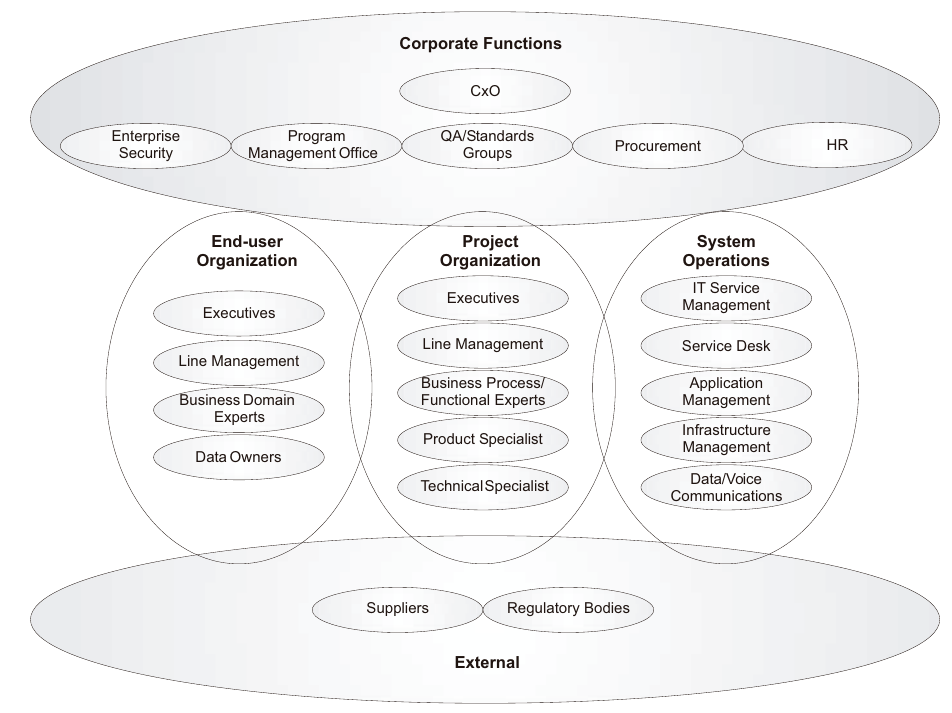
\includegraphics[width=\textwidth]{../figures/sample_stakeholders}
	\end{minipage}
	\hfill
	\begin{minipage}[bt]{0.496\textwidth}
		\centering
		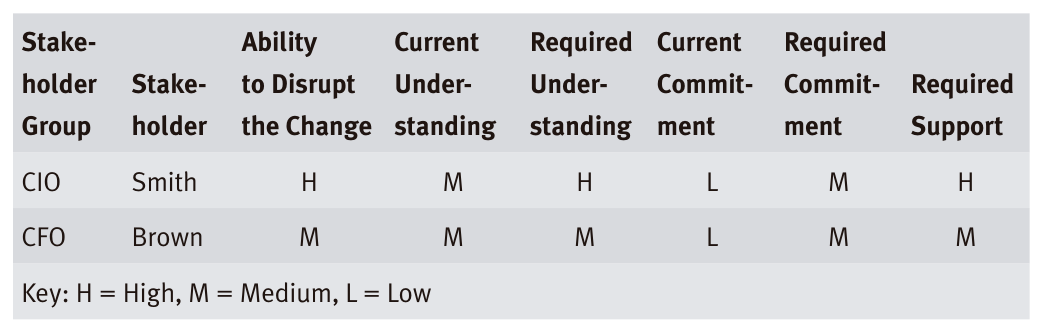
\includegraphics[width=\textwidth]{../figures/stakeholder_analysis}
		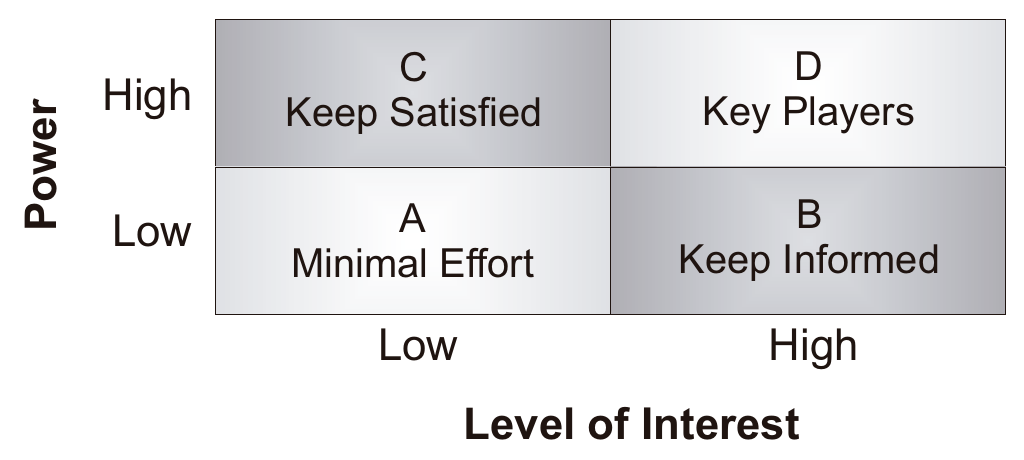
\includegraphics[width=\textwidth]{../figures/power_vs_interest}
	\end{minipage}
	\caption{Contoh Pemangku Kepentingan, Analisis Pemangku Kepentingan, Kekuatan vs Kepentingan}
	\label{fig:stakeholders}
\end{figure}

\subsection{Contoh Pemangku Kepentingan (Stakeholders)}
Dalam konteks transformasi menjadi hybrid working di Universitas ABC, pemangku kepentingan terbagi ke dalam beberapa kelompok, yang masing-masing memiliki peran dan tanggung jawab yang berbeda. Kelompok pemangku kepentingan tersebut meliputi:

\begin{itemize}
	\item \textbf{Corporate Functions:} 
	Fungsi korporat bertanggung jawab atas kebijakan dan strategi umum universitas. Contoh jabatan dalam kelompok ini meliputi Rektor, Wakil Rektor Bidang Akademik, dan Direktur Keuangan.
	
	\item \textbf{End-User Organization:} 
	Organisasi pengguna akhir terdiri dari mahasiswa dan dosen yang akan menggunakan sistem baru. Jabatan yang termasuk dalam kelompok ini antara lain Mahasiswa, Dosen, Pengajar dan Asisten Dosen.
	
	\item \textbf{Project Organization:} 
	Organisasi proyek terdiri dari tim yang terlibat dalam perencanaan dan pelaksanaan proyek transformasi. Jabatan yang ada dalam kelompok ini termasuk Manajer Proyek, Tim Arsitektur, Analis Bisnis, dan Tim Pengembangan TI.
	
	\item \textbf{System Operations:} 
	Tim operasi sistem bertanggung jawab untuk menjaga agar sistem berjalan dengan baik setelah implementasi. Jabatan dalam kelompok ini meliputi Administrator Sistem, Staf Dukungan TI, dan Teknisi Jaringan.
	
	\item \textbf{External:} 
	Pemangku kepentingan eksternal mencakup pihak-pihak yang berada di luar universitas tetapi berpengaruh terhadap proyek. Contoh jabatan dalam kelompok ini termasuk Vendor Teknologi, Konsultan Pendidikan, dan Badan Akreditasi.
\end{itemize}

\subsection{Analisis Kontribusi dan Kepentingan Posisi dalam Organisasi}

Dalam konteks transformasi hybrid working di universitas, analisis kontribusi dan kepentingan posisi dalam organisasi sangat penting untuk memastikan keberhasilan implementasi. Berikut adalah beberapa posisi kunci beserta analisisnya:

\begin{itemize}
	\item \textbf{Pimpinan Universitas (Rektor)}: 
	Memiliki kemampuan untuk mendisrupsi perubahan signifikan melalui pengambilan keputusan strategis dan penyediaan sumber daya. Pemahaman saat ini terhadap permasalahan dan solusi perlu dievaluasi, serta komitmen mereka untuk mendukung inisiatif hybrid working sangat penting.
	
	\item \textbf{Dekan Fakultas}: 
	Berperan sebagai penghubung antara kebijakan universitas dan kebutuhan program studi. Saat ini, mereka mungkin sudah memiliki pemahaman yang baik tentang permasalahan di tingkat fakultas. Namun, komitmen mereka untuk mendukung inisiatif ini perlu ditingkatkan agar dapat memberikan dukungan yang lebih besar kepada dosen dan mahasiswa.
	
	\item \textbf{Tim TI (Kepala IT)}: 
	Bertanggung jawab untuk mengeksekusi solusi teknis dan memastikan infrastruktur mendukung kebutuhan hybrid working. Tingkat dukungan yang mereka perlukan harus dinilai berdasarkan kemampuan mereka dalam menghadapi tantangan teknis. Peningkatan pemahaman mereka terhadap solusi yang akan diterapkan melalui pelatihan tambahan sangat diperlukan.
	
	\item \textbf{Mahasiswa}: 
	Sebagai pengguna akhir, pemahaman mereka tentang sistem baru yang akan mendukung pembelajaran hybrid perlu diperkuat. Tingkat dukungan yang diperlukan dari mereka dapat ditingkatkan melalui sosialisasi dan pelatihan mengenai teknologi baru, untuk memastikan adopsi dan komitmen terhadap perubahan.
\end{itemize}


\subsection{Penggunaan Kuadran Power dan Level of Interest}

Dalam analisis pemangku kepentingan untuk transformasi hybrid working di universitas, penggunaan kuadran kekuasaan (power) dan tingkat minat (interest) sangat penting untuk mengidentifikasi posisi-posisi kunci dan pendekatan yang tepat dalam melibatkan mereka. Kuadran ini dibagi menjadi empat kategori:

\begin{itemize}
	\item \textbf{Kuadran I: High Power, High Interest}
	\begin{itemize}
		\item \textbf{Contoh: Rektor}
		\item Rektor memiliki kekuasaan tinggi dalam pengambilan keputusan strategis dan juga sangat tertarik dengan keberhasilan transformasi hybrid working. Pendekatan yang tepat adalah memastikan komunikasi yang sering dan keterlibatan langsung dalam proses perencanaan dan implementasi.
	\end{itemize}
	
	\item \textbf{Kuadran II: High Power, Low Interest}
	\begin{itemize}
		\item \textbf{Contoh: Dewan Pengurus Universitas}
		\item Meskipun memiliki kekuasaan tinggi, mereka mungkin tidak memiliki ketertarikan yang mendalam terhadap detail operasional transformasi. Oleh karena itu, pendekatan yang efektif adalah memberikan informasi berkala yang relevan, serta memastikan bahwa keputusan strategis mereka sejalan dengan tujuan transformasi.
	\end{itemize}
	
	\item \textbf{Kuadran III: Low Power, High Interest}
	\begin{itemize}
		\item \textbf{Contoh: Mahasiswa}
		\item Mahasiswa mungkin tidak memiliki kekuasaan dalam pengambilan keputusan, tetapi mereka memiliki ketertarikan tinggi terhadap inisiatif yang mempengaruhi pengalaman belajar mereka. Untuk itu, penting untuk melibatkan mereka melalui forum diskusi, survei, dan pelatihan agar mereka merasa diikutsertakan dalam proses transformasi.
	\end{itemize}
	
	\item \textbf{Kuadran IV: Low Power, Low Interest}
	\begin{itemize}
		\item \textbf{Contoh: Staf Administrasi yang Tidak Terlibat Langsung}
		\item Posisi ini memiliki kekuasaan dan ketertarikan rendah terhadap proyek. Pendekatan yang diperlukan adalah minimal, hanya memberikan informasi yang diperlukan agar mereka tetap terinformasi tanpa membebani mereka dengan detail yang tidak relevan.
	\end{itemize}
\end{itemize}

Dengan memahami posisi masing-masing pemangku kepentingan dalam kuadran ini, universitas dapat mengembangkan strategi komunikasi dan keterlibatan yang lebih efektif untuk mendukung keberhasilan transformasi hybrid working.


\section{Peta Pemangku Kepentingan}
Lihat Gambar \ref{fig:stakeholders_map}.
\begin{figure}[h!]
	\centering
	\begin{minipage}[bt]{0.496\textwidth}
		\centering
		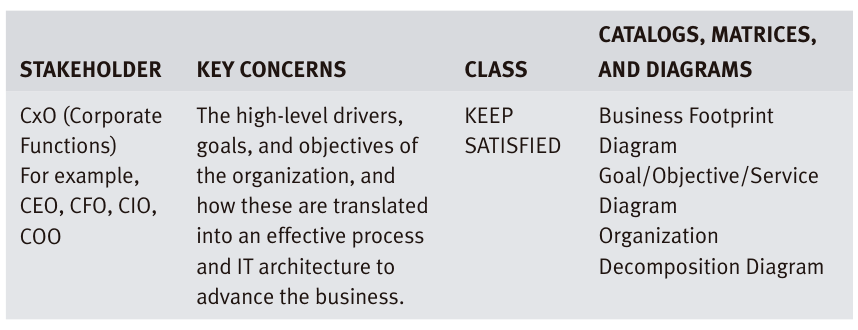
\includegraphics[width=\textwidth]{../figures/stakeholder_map_1}
		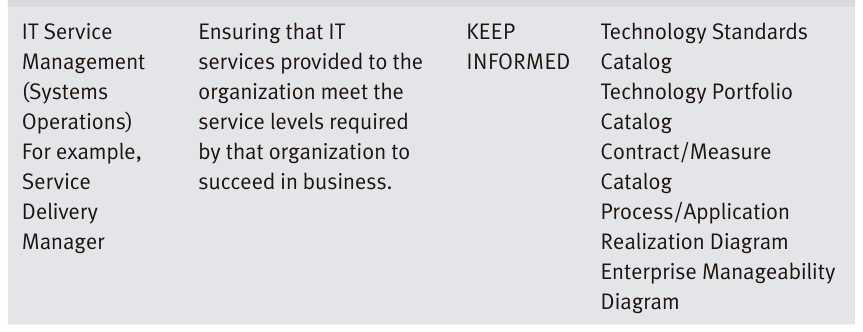
\includegraphics[width=\textwidth]{../figures/stakeholder_map_3}
	\end{minipage}
	\hfill
	\begin{minipage}[bt]{0.496\textwidth}
		\centering
		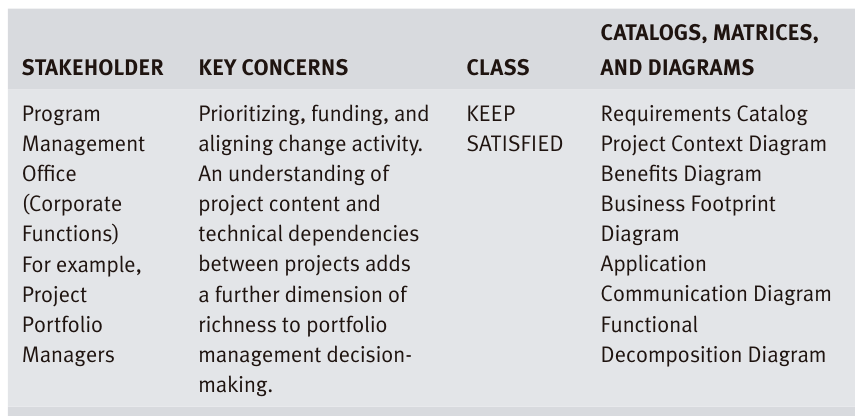
\includegraphics[width=\textwidth]{../figures/stakeholder_map_2}
	\end{minipage}
	\caption{Peta Pemangku Kepentingan}
	\label{fig:stakeholders_map}
\end{figure}


\subsection*{Contoh Keterkaitan antara Posisi Stakeholders dan Pola Komunikasi}

Keterkaitan antara posisi pemangku kepentingan dalam organisasi, keprihatinan utama mereka, dan pola komunikasi yang diterapkan adalah faktor penting dalam memastikan keberhasilan transformasi hybrid working di universitas. Berikut adalah analisis keterkaitan tersebut:

\begin{itemize}
	\item \textbf{Posisi Stakeholders dan Keprihatinan Utama}
	\begin{itemize}
		\item \textbf{Rektor (High Power, High Interest):} Rektor memiliki keprihatinan terhadap hasil akhir dari transformasi. Mereka fokus pada peningkatan pengalaman belajar mahasiswa dan efektivitas pengajaran.
		\item \textbf{Dekan Fakultas (High Power, Low Interest):} Dekan perlu memastikan bahwa kebijakan yang diterapkan sejalan dengan visi akademis, meskipun tidak terlibat dalam detail teknis. 
		\item \textbf{Mahasiswa (Low Power, High Interest):} Mahasiswa sangat peduli dengan aksesibilitas dan kualitas pembelajaran, yang langsung berdampak pada pengalaman belajar mereka.
		\item \textbf{Staf Administrasi (Low Power, Low Interest):} Mereka membutuhkan informasi yang cukup untuk mendukung kegiatan sehari-hari, namun tidak memerlukan keterlibatan mendalam.
	\end{itemize}
	
	\item \textbf{Pola Komunikasi}
	\begin{itemize}
		\item \textbf{Keep Satisfied:} Untuk pemangku kepentingan seperti Dewan Pengurus Universitas, penting untuk memberikan informasi strategis secara berkala, sehingga mereka merasa dilibatkan tanpa terlalu mendalami rincian proyek.
		\item \textbf{Key Players:} Rektor dan tim arsitektur harus berkomunikasi secara langsung dan rutin, menjaga mereka terinformasi tentang kemajuan dan tantangan dalam proyek.
		\item \textbf{Minimal Efforts:} Staf administrasi hanya perlu mendapatkan pembaruan dasar yang relevan untuk menjalankan tugas mereka tanpa detail tambahan.
		\item \textbf{Keep Informed:} Mahasiswa perlu mendapatkan informasi yang cukup mengenai perubahan yang akan mempengaruhi mereka, seperti pelatihan penggunaan platform baru dan cara berpartisipasi dalam feedback.
	\end{itemize}
	
	\item \textbf{Kaitannya dengan Alat-Alat Komunikasi di TOGAF}
	\begin{itemize}
		\item \textbf{Catalogs:} Penggunaan catalogs dapat membantu dalam menyusun daftar pemangku kepentingan, termasuk peran, keprihatinan utama, dan pola komunikasi yang diperlukan untuk masing-masing. Contoh: \textit{Stakeholder Catalog} yang merinci nama, jabatan, dan keprihatinan mereka.
		\item \textbf{Matrices:} Matriks keterkaitan antara pemangku kepentingan dan keprihatinan mereka dapat memberikan gambaran visual tentang siapa yang perlu dihubungi untuk isu tertentu. Contoh: \textit{Stakeholder Analysis Matrix} yang menghubungkan pemangku kepentingan dengan pola komunikasi dan jenis informasi yang dibutuhkan.
		\item \textbf{Diagrams:} Diagram alur dapat digunakan untuk menggambarkan pola komunikasi antar pemangku kepentingan, menunjukkan aliran informasi dan bagaimana setiap kelompok berinteraksi. Contoh: \textit{Communication Flow Diagram} yang menggambarkan interaksi antara rektor, dekan, dan mahasiswa dalam proses pengambilan keputusan.
	\end{itemize}
\end{itemize}

Dengan memahami keterkaitan posisi, keprihatinan, dan pola komunikasi yang sesuai, universitas dapat memastikan semua pemangku kepentingan terlibat secara efektif dalam proses transformasi hybrid working, menggunakan alat-alat komunikasi yang tepat untuk mendukung tujuan tersebut.


\section{Menilai Kesiapan untuk Transformasi}
\label{sec:kesiapan_transformasi}
\begin{itemize}
	\item Visi.
	\item Keinginan atau kesediaan untuk mencapai hasil.
	\item Persyaratan.
	\item Adanya indikasi/kasus dalam bisnis.
	\item Dana.
	\item Sponsorship dan kepemimpinan.
	\item Tata kelola.
	\item Akuntabilitas (kemampuan untuk dipertanggungjawabkan).
	\item Pendekatan dan model eksekusi yang dapat diterapkan.
	\item Kapasitas IT untuk mengeksekusi.
	\item Kapasitas perusahaan untuk mengeksekusi.
	\item Kemampuan perusahaan untuk mengimplementasikan dan mengoperasikan pasca eksekusi.
\end{itemize}

\subsection*{Contoh Menilai Kesiapan untuk Transformasi:}
\begin{itemize}
	\item \textbf{Visi.} Visi transformasi adalah untuk menciptakan pengalaman belajar hybrid yang terintegrasi, di mana mahasiswa dapat belajar secara fleksibel dan efisien, dengan dukungan teknologi yang memadai dan aksesibilitas yang tinggi.
	
	\item \textbf{Keinginan atau kesediaan untuk mencapai hasil.} Universitas ABC menunjukkan keinginan yang kuat untuk mencapai hasil yang diinginkan, yaitu peningkatan keterlibatan mahasiswa dan efektivitas pengajaran, dengan dukungan dari berbagai pemangku kepentingan.
	
	\item \textbf{Persyaratan (\textit{Requirements}).} Persyaratan untuk transformasi mencakup kebutuhan akan infrastruktur teknologi yang kuat, platform pembelajaran yang interaktif, dan pelatihan untuk dosen serta staf dalam penggunaan teknologi baru.
	
	\item \textbf{Adanya indikasi/kasus dalam bisnis.} Indikasi adanya kebutuhan untuk transformasi terlihat dari umpan balik mahasiswa yang menunjukkan ketidakpuasan terhadap pengalaman pembelajaran hybrid yang ada saat ini, serta meningkatnya permintaan untuk metode pembelajaran yang lebih fleksibel.
	
	\item \textbf{Dana.} Universitas telah mengalokasikan anggaran khusus untuk mendukung proyek transformasi ini, termasuk dana untuk pengembangan teknologi, pelatihan, dan peningkatan infrastruktur.
	
	\item \textbf{Sponsorship dan kepemimpinan.} Proyek ini didukung oleh pimpinan universitas, termasuk rektor dan dekan fakultas, yang berkomitmen untuk menyediakan sumber daya dan dukungan yang diperlukan untuk keberhasilan transformasi.
	
	\item \textbf{Tata kelola.} Proyek akan dikelola melalui komite pengawasan proyek yang terdiri dari perwakilan dari berbagai fakultas dan unit administrasi, memastikan bahwa semua aspek transformasi terkoordinasi dengan baik.
	
	\item \textbf{Akuntabilitas (kemampuan untuk dipertanggungjawabkan).} Setiap pemangku kepentingan akan memiliki peran dan tanggung jawab yang jelas dalam proyek, dengan mekanisme untuk menilai dan mempertanggungjawabkan kemajuan yang dicapai.
	
	\item \textbf{Pendekatan dan model eksekusi yang dapat diterapkan.} Pendekatan agile akan digunakan untuk memastikan bahwa transformasi dapat beradaptasi dengan kebutuhan yang berubah dan memberikan hasil yang cepat serta iteratif.
	
	\item \textbf{Kapasitas IT untuk mengeksekusi.} Tim TI universitas memiliki keterampilan dan pengalaman yang diperlukan untuk mendukung pengembangan dan implementasi sistem teknologi yang diperlukan untuk transformasi.
	
	\item \textbf{Kapasitas perusahaan untuk mengeksekusi.} Universitas memiliki kapasitas yang cukup dalam hal sumber daya manusia dan infrastruktur untuk melaksanakan transformasi ini, dengan adanya dukungan dari berbagai fakultas dan unit.
	
	\item \textbf{Kemampuan perusahaan untuk mengimplementasikan dan mengoperasikan pasca eksekusi.} Setelah implementasi, universitas akan membentuk tim dukungan untuk memastikan bahwa semua sistem dan proses baru dapat beroperasi dengan lancar, serta memberikan pelatihan berkelanjutan kepada dosen dan staf.
\end{itemize}


\section{Visi Arsitektur}
\label{sec:visi_arsitektur}
\begin{itemize}
	\item Deskripsi masalah, termasuk pemangku kepentingan dan kekhawatiran mereka, serta daftar masalah/skenario yang perlu diatasi.
	\item Tujuan dari \textit{Architectural Work Statement}.
	\item Ringkasan pandangan yang diperlukan untuk Arsitektur tingkat tinggi dan Permintaan Pekerjaan Arsitektur Bisnis, Aplikasi, Data, dan Teknologi.
	\item Skenario bisnis.
	\item Kebutuhan pemangku kepentingan yang telah dipetakan dan dirinci.
\end{itemize}

\subsection*{Contoh Visi Arsitektur:}
\begin{itemize}
	\item \textbf{Deskripsi masalah}. Universitas ABC menghadapi tantangan dalam memberikan pengalaman belajar yang terintegrasi antara mode pembelajaran fisik dan daring. Pemangku kepentingan yang terlibat, termasuk mahasiswa, dosen, dan staf administrasi, memiliki kekhawatiran terkait aksesibilitas materi pembelajaran, keterlibatan mahasiswa dalam kelas hybrid, dan efisiensi penggunaan teknologi. Masalah yang perlu diatasi mencakup:
	\begin{itemize}
		\item Kurangnya aksesibilitas teknologi untuk mahasiswa yang belajar dari rumah.
		\item Kesulitan dalam kolaborasi antara mahasiswa yang hadir secara fisik dan yang berpartisipasi secara daring.
		\item Ketidakpuasan mahasiswa terhadap pengalaman belajar hybrid.
	\end{itemize}
	
	\item \textbf{Tujuan dari \textit{Architectural Work Statement}}. Tujuan dari dokumen ini adalah untuk merumuskan strategi arsitektur yang mendukung implementasi pembelajaran hybrid di Universitas ABC, memastikan bahwa semua pemangku kepentingan memiliki akses yang setara terhadap materi pembelajaran dan dapat berpartisipasi dalam interaksi akademik secara efektif.
	
	\item \textbf{Ringkasan pandangan}. Visi arsitektur tingkat tinggi mencakup integrasi sistem informasi akademik dengan platform kolaborasi untuk menciptakan lingkungan belajar yang seamless. Permintaan pekerjaan arsitektur mencakup pengembangan solusi di area Bisnis, Aplikasi, Data, dan Teknologi, dengan fokus pada:
	\begin{itemize}
		\item \textbf{Bisnis:} Meningkatkan pengalaman belajar mahasiswa dan keterlibatan dosen dalam kelas hybrid.
		\item \textbf{Aplikasi:} Pengembangan aplikasi pembelajaran yang mendukung interaksi real-time.
		\item \textbf{Data:} Penyediaan data analitik untuk melacak keterlibatan dan kinerja mahasiswa.
		\item \textbf{Teknologi:} Penyediaan infrastruktur teknologi yang handal untuk mendukung pembelajaran hybrid.
	\end{itemize}
	
	\item \textbf{Skenario bisnis}. Proyek ini bertujuan untuk memperkuat keterhubungan antara mahasiswa yang belajar secara daring dan luring, mengoptimalkan penggunaan ruang kelas dengan teknologi terbaru, dan menciptakan metode pembelajaran yang adaptif untuk memenuhi kebutuhan mahasiswa dari berbagai latar belakang.
	
	\item \textbf{Kebutuhan pemangku kepentingan yang telah dipetakan dan dirinci}. Kebutuhan pemangku kepentingan mencakup:
	\begin{itemize}
		\item \textbf{Mahasiswa:} Akses mudah ke materi pembelajaran dan dukungan teknis yang memadai.
		\item \textbf{Dosen:} Alat yang memungkinkan pengajaran efektif di kelas hybrid dan dukungan dalam mengevaluasi kinerja mahasiswa.
		\item \textbf{Staf Administrasi:} Sistem untuk memantau keterlibatan mahasiswa dan efektivitas program hybrid.
	\end{itemize}
	Setiap kebutuhan akan dipetakan ke dalam rencana implementasi untuk memastikan bahwa solusi arsitektur memenuhi harapan semua pemangku kepentingan.
\end{itemize}

\section{Skenario Bisnis}
\label{sec:skenario_bisnis}
\begin{itemize}
	\item \textbf{Masalah}. Mengidentifikasi, mendokumentasikan, dan memberi peringkat pada masalah yang menjadi pendorong proyek.
	\item \textbf{Lingkungan Bisnis dan Teknis}. Mendokumentasikan sebagai model arsitektur tingkat tinggi lingkungan bisnis dan teknis di mana situasi masalah terjadi.
	\item \textbf{Tujuan dan Ukuran Keberhasilan}. Mengidentifikasi dan mendokumentasikan tujuan yang diharapkan, hasil dari penyelesaian masalah yang berhasil.
	\item \textbf{Aktor Manusia}. Mengidentifikasi aktor manusia dan peran mereka dalam model bisnis, partisipan manusia, dan perannya.
	\item \textbf{Aktor Komputer}. Mengidentifikasi aktor komputer dan peran mereka dalam model teknologi, elemen komputasi, dan perannya.
	\item \textbf{Peran dan Tanggung Jawab}. Mengidentifikasi dan mendokumentasikan peran, tanggung jawab, dan ukuran keberhasilan setiap aktor, skrip yang dibutuhkan setiap aktor, dan hasil yang diharapkan dari penanganan situasi yang tepat.
	\item \textbf{Revisi}. Memeriksa kesesuaian tujuan untuk menginspirasi pekerjaan arsitektur selanjutnya, dan menyempurnakan hanya jika diperlukan.
\end{itemize}

\subsection*{Contoh Skenario Bisnis:}
\begin{itemize}
	\item \textbf{Masalah}. Universitas ABC menghadapi tantangan dalam menyediakan pengalaman belajar yang seimbang antara interaksi fisik dan digital, dengan meningkatnya jumlah mahasiswa yang memilih model pembelajaran hybrid. Masalah ini mencakup kurangnya infrastruktur teknologi yang mendukung, kesulitan dalam kolaborasi antara mahasiswa, dan perbedaan dalam aksesibilitas materi pembelajaran.
	
	\item \textbf{Lingkungan Bisnis dan Teknis}. Lingkungan bisnis mencakup semua fakultas di Universitas ABC, yang melayani mahasiswa dari berbagai latar belakang. Lingkungan teknis melibatkan platform pembelajaran daring (misalnya, Learning Management System), alat kolaborasi (seperti Microsoft Teams), serta perangkat keras di ruang kelas seperti proyektor dan sistem audio untuk mendukung interaksi daring dan luring.
	
	\item \textbf{Tujuan dan Ukuran Keberhasilan}. Tujuan dari proyek ini adalah meningkatkan pengalaman belajar mahasiswa dengan menyediakan platform yang memungkinkan kolaborasi efektif antara mahasiswa yang hadir secara fisik dan daring. Ukuran keberhasilan dapat diukur melalui survei kepuasan mahasiswa, peningkatan partisipasi dalam kelas, dan evaluasi hasil akademik yang menunjukkan peningkatan minimal 15\% dalam nilai akhir mahasiswa.
	
	\item \textbf{Aktor Manusia}. Aktor manusia yang terlibat dalam model bisnis ini mencakup:
	\begin{itemize}
		\item \textbf{Mahasiswa:} Menghadiri kelas baik secara daring maupun luring dan berkolaborasi dalam proyek.
		\item \textbf{Dosen:} Mengajar dan memfasilitasi interaksi antara mahasiswa di kelas fisik dan virtual.
		\item \textbf{Staf TI:} Menyediakan dukungan teknis dan pemeliharaan sistem teknologi yang digunakan.
	\end{itemize}
	
	\item \textbf{Aktor Komputer}. Aktor komputer dalam model teknologi mencakup:
	\begin{itemize}
		\item \textbf{Platform Pembelajaran Daring:} Sistem yang digunakan untuk menyampaikan materi pembelajaran dan memfasilitasi interaksi.
		\item \textbf{Alat Kolaborasi:} Alat yang digunakan untuk komunikasi dan kolaborasi, seperti Microsoft Teams dan Google Meet.
		\item \textbf{Sistem Manajemen Data:} Database yang menyimpan informasi tentang mahasiswa, dosen, dan materi pembelajaran.
	\end{itemize}
	
	\item \textbf{Peran dan Tanggung Jawab}. Peran dan tanggung jawab setiap aktor mencakup:
	\begin{itemize}
		\item \textbf{Mahasiswa:} Berpartisipasi aktif dalam kelas, memberikan umpan balik mengenai pengalaman belajar.
		\item \textbf{Dosen:} Menyusun materi pembelajaran yang sesuai untuk format hybrid dan mengevaluasi partisipasi serta kinerja mahasiswa.
		\item \textbf{Staf TI:} Memastikan semua alat dan platform berjalan dengan baik, memberikan pelatihan teknis kepada dosen dan mahasiswa.
	\end{itemize}
	Ukuran keberhasilan setiap aktor dapat diukur melalui kinerja individu dan umpan balik dari pemangku kepentingan lainnya.
	
	\item \textbf{Revisi}. Revisi dilakukan secara berkala berdasarkan umpan balik dari mahasiswa dan dosen untuk memastikan bahwa tujuan proyek tetap relevan dan inspiratif untuk pengembangan arsitektur lebih lanjut. Jika diperlukan, langkah-langkah dapat disempurnakan untuk meningkatkan efektivitas pelaksanaan pembelajaran hybrid.
\end{itemize}


\section{Dokumen \textit{Architectural Statement of Work}}
\label{sec:stament_of_work}
\begin{itemize}
	\item Judul.
	\item Permintaan Proyek Arsitektur dan Latar Belakang.
	\item Deskripsi Proyek Arsitektur dan Ruang Lingkup.
	\item Ikhtisar Visi Arsitektur.
	\item Prosedur Khusus Perubahan Ruang Lingkup.
	\item Peran, Tanggung Jawab, dan Deliverables.
	\item Kriteria dan Prosedur Penerimaan.
	\item Rencana dan Jadwal Proyek Arsitektur.
	\item Persetujuan.
\end{itemize}

\subsection*{Contoh Dokumen:}
\begin{itemize}
	\item \textbf{Judul.} 
	Architectural Statement of Work untuk Implementasi Hybrid Working di Universitas ABC.
	
	\item \textbf{Permintaan Proyek Arsitektur dan Latar Belakang.} 
	Permintaan untuk proyek arsitektur ini muncul dari kebutuhan Universitas ABC untuk menyediakan lingkungan belajar yang fleksibel dan mendukung pembelajaran hybrid sebagai respon terhadap perubahan dalam cara mahasiswa belajar yang terjadi akibat pandemi COVID-19 dan perkembangan teknologi pendidikan.
	
	\item \textbf{Deskripsi Proyek Arsitektur dan Ruang Lingkup.} 
	Proyek ini bertujuan untuk merancang dan mengimplementasikan sistem yang mendukung pembelajaran hybrid, mencakup pengembangan platform kolaborasi seperti Microsoft Teams dan Zoom, integrasi sistem informasi akademik seperti SIAKAD, serta perancangan ulang ruang kelas untuk mendukung interaksi daring dan luring dengan menggunakan teknologi proyeksi dan alat interaksi digital.
	
	\item \textbf{Ikhtisar Visi Arsitektur.} 
	Visi arsitektur adalah menciptakan pengalaman belajar yang seamless antara interaksi fisik dan digital, memungkinkan mahasiswa untuk mengakses materi pembelajaran secara daring, berkolaborasi dengan sesama mahasiswa dalam proyek kelompok, dan berinteraksi dengan dosen melalui sesi tatap muka dan daring secara fleksibel.
	
	\item \textbf{Prosedur Khusus Perubahan Ruang Lingkup.} 
	Prosedur untuk perubahan ruang lingkup meliputi pengajuan permintaan tertulis oleh pemangku kepentingan seperti dosen dan mahasiswa, evaluasi dampak perubahan oleh tim arsitektur, serta persetujuan perubahan oleh komite pengawasan proyek yang terdiri dari perwakilan fakultas dan IT.
	
	\item \textbf{Peran, Tanggung Jawab, dan Deliverables.} 
	Peran dalam proyek ini mencakup:
	\begin{itemize}
		\item \textbf{Manajer Proyek:} Bertanggung jawab untuk pengelolaan keseluruhan proyek dan komunikasi dengan pemangku kepentingan.
		\item \textbf{Tim Arsitektur:} Bertanggung jawab untuk perancangan solusi teknis dan strategi implementasi.
		\item \textbf{Staf TI:} Bertanggung jawab untuk implementasi teknis, pemeliharaan, dan dukungan sistem.
	\end{itemize}
	Deliverables mencakup dokumen perancangan yang detail, prototipe sistem, dan laporan kemajuan proyek yang disampaikan setiap bulan.
	
	\item \textbf{Kriteria dan Prosedur Penerimaan.} 
	Kriteria penerimaan mencakup penyelesaian proyek sesuai dengan spesifikasi yang disepakati, serta hasil evaluasi pengguna yang menunjukkan tingkat kepuasan yang tinggi (minimal 80\%). Prosedur penerimaan melibatkan pengujian fungsional dan evaluasi oleh pemangku kepentingan setelah fase implementasi.
	
	\item \textbf{Rencana dan Jadwal Proyek Arsitektur.} 
	Rencana proyek mencakup fase-fase utama seperti perencanaan (2 bulan), desain (1 bulan), implementasi (3 bulan), dan evaluasi (1 bulan). Jadwal proyek akan dibagi menjadi beberapa milestone, dengan estimasi waktu untuk masing-masing fase, di mana setiap fase akan dievaluasi pada akhir periode masing-masing.
	
	\item \textbf{Persetujuan.} 
	Dokumen ini memerlukan persetujuan dari pemangku kepentingan utama, termasuk Rektor Universitas ABC, Dekan Fakultas Ilmu Komputer, dan perwakilan mahasiswa, sebelum proyek dapat dilanjutkan ke fase berikutnya.
\end{itemize}


\section{Ringkasan}
\begin{itemize}
	\item Fase \textit{Architectural Vision} adalah langkah pertama dalam Metode Pengembangan Arsitektur TOGAF, di mana ruang lingkup didefinisikan, pemangku kepentingan diidentifikasi, dan visi arsitektur tingkat tinggi ditetapkan.
	\item Fase ini penting untuk memastikan bahwa proyek arsitektur memiliki dukungan dan arahan yang tepat sejak awal.
\end{itemize}

\section{Kegiatan Kelas dan Tugas}
Buatlah visi untuk kapabilitas arsitektur yang Anda pilih, berdasarkan informasi yang dikumpulkan dalam fase Preliminary dan fase ini. Deskripsikan keadaan saat ini (As-Is) dan keadaan target (To-Be) untuk memperjelas visi arsitektur tersebut dalam bentuk kajian kesiapan (Subbab \ref{sec:kesiapan_transformasi}), kajian \textit{stakeholders} (Subbab \ref{sec:stakholders}), perumusan visi arsitektur (Subbab \ref{sec:visi_arsitektur}), kajian skenario bisnis (Subbab \ref{sec:skenario_bisnis}), dan dokumen \textit{Architectural Statement of Work}(Subbab \ref{sec:stament_of_work}).
